% %%%%%%%%%%%%%%%%%%%%%%%%%%%%%%%%%%%%%%%%%%%%%%%%%%%%%%%%%%%%%%%%%%%%%%
%  ╭─────────╮                      ╔══╦╗ ╗ ╔═╦═╗ ╥ ┌─┐┌─┐┌─┐┬ ┬┌─┐┌┐ ┬
%  │ ,-= ━━━┑│                  |   ╠═╦╝╚╗╠╗║ ║ ╠═╣ ├─┤├─┤│  ├─┤├─ │└┐│
%  │ % iTec  │                  |   ╨ ╚═ ╚╝╚╝ ╨ ╨ ╨ ┴ ┴┴ ┴└─┘┴ ┴└─┘┴ └┘
%  │┃°. .°.  │ Chair Individual |          ┬ ┬┌┐ ┬┬┬  ┬┌─┐┬─┐┌─┐┬┌┬┐┬ ┬
%  │┖  °   ° │   and Technology |          │ ││└┐││└┐┌┘├─ ├┬┘└─┐│ │ └┬┘
%  ╰─────────╯                             └─┘┴ └┘┴ └┘ └─┘┴└─└─┘┴ ┴  ┴
% %%%%%%%%%%%%%%%%%%%%%%%%%%%%%%%%%%%%%%%%%%%%%%%%%%%%%%%%%%%%%%%%%%%%%%
%  This file is part of the Master's thesis LaTeX template used at the
%  Chair Individual and Technology (iTec) at RWTH Aachen University.
% %%%%%%%%%%%%%%%%%%%%%%%%%%%%%%%%%%%%%%%%%%%%%%%%%%%%%%%%%%%%%%%%%%%%%%


%% %%%%%%%%%%%%%%%%%%%%%%%%%%%%%%%%%%%%%%%%%%%%%%%%%%%%%%%%%%%%%%%%%%%%%
\chapter{(Theoretical) Background and Related Work}
\label{chap:background_related-work}


\section{Large Language Models}
\label{sec:llm}
\subsection{Model architecture}
Large Language Models (LLMs) are machine leaning models based on the Transformer Architecture which was first introduced by \citet{vaswani2017attention} and came proceeding developments in sequence modelling such as LSTMs \citep{hochreiter1997long} and (gated) Recurrent Neural Networks (RNN) \citep{cho2014learning}. Transformer models rely completely on self-attention to compute representations of its input and output without using sequence-aligned RNNs or convolutions. These leads to major gains with regards to the parallelisation of computation and long-range dependencies of the input text \cite{kimDHR17}. 

In this process of exploring RNNs for machine translation and text summarisation the concept encoder-decoder structure was developed \cite{sutskever2014sequence}. The encoders will take the input being a embedding sequence $X$ which consists of the input and the positional encoding and creates an intermediate vector $Z$ which can then be processed by the decoder. Additionally the decoder will also get the previously self-generated output token as an input.


Building on the transformer architecture \citep{radford2018improving} created a new approach using the unsupervised pre-training + supervised fine-tuning paradigm. This is done by applying a generative pre-training on a the transformer, which is then followed by a discriminative fine-tuning on a specific task. The advantage of this was that due to the model already having the casual relationships inside one was able to fine-tune the model with a lot smaller datasets. Combining unsupervised with supervised techniques is in itself not novel and has already previously been used for sequence labelling or text classification \cite{van2020survey, yarowsky1995unsupervised}.


Unlike encoder-decoder models, which process the entire input before generating output, GPT models rely only on a decoder with causal masking. This allows them to generate text sequentially while maintaining coherence over long contexts \ref{fig:decoder} \cite{radford2018improving,brown2020language}. The decoder will given sequence of tokens $(x_{i-k},...,x_{i-1})$ predict or classify token $x_i$. 


\begin{figure}
    \centering
    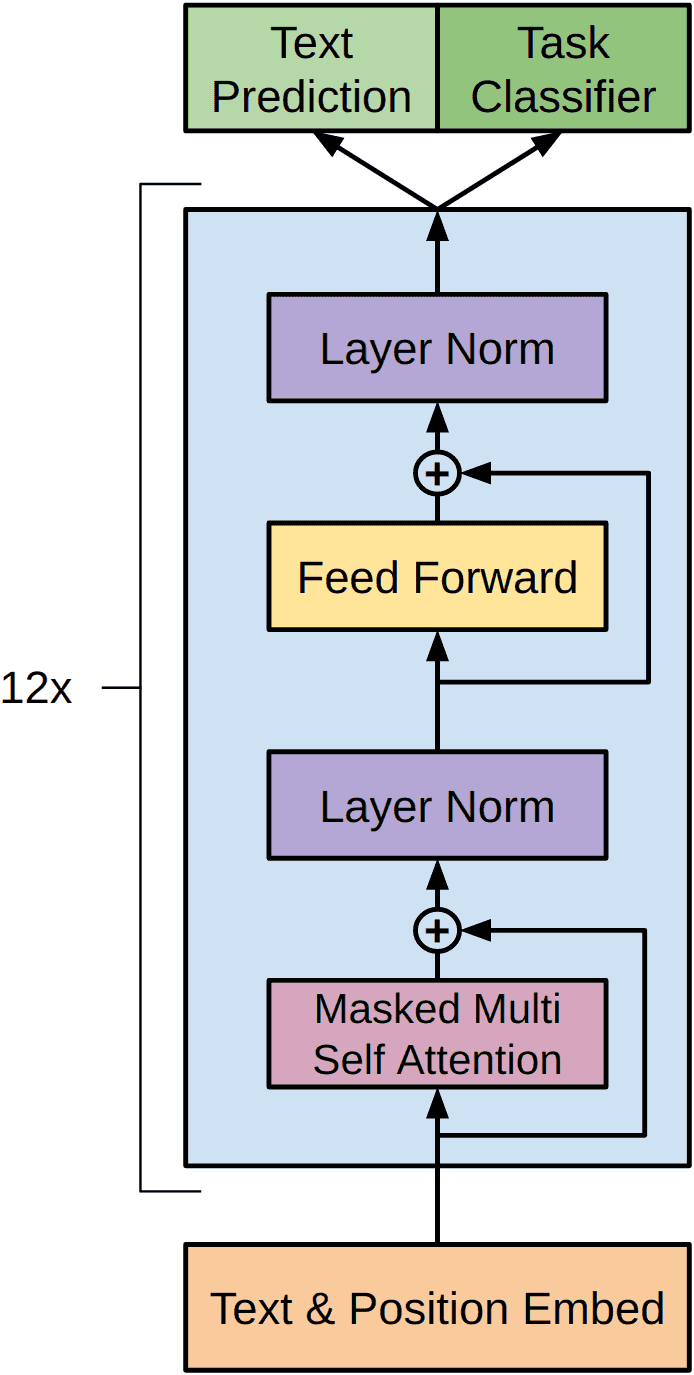
\includegraphics[width=0.5\linewidth]{imgs/decoder.png}
    \caption{Decoder structure proposed by \citet{radford2018improving}}
    \label{fig:decoder}
\end{figure}



The attention mechanism contains 
The mentioned attention is symbolised by the formula \ref{for:attention}, where Q is the query, K is the Key and V is is value. 
\begin{align}
\label{for:attention}
    \text{Attention}(Q,K,V) &= softmax(\frac{QK^T}{\sqrt{d_k}})V
\end{align}


Rather then just having a single attention \cite{vaswani2017attention} create a concept called multi-headed-attention which can be seen in formula \ref{for:multiHead}. Having a multi-headed-attention allows for different attention heads to focus on different aspects of the input. This type of model also allows for highly parallelised training and inference of the data \citep{min2023recent}. 

\begin{align}
\label{for:multiHead}
    \text{MultiHead}(Q,K,V) &= Concat(head_1, head_2 ... , head_h)W^0 \\
    \text{where head}_i &= \text{Attention}(QW_i^Q,KW^K_i, VW^V_i)
\end{align}



\subsection{Alignment fine tuning RLTH}
\label{sub:alignment}

When using LLMs for generating text they will in their pre fine-tuned state find the token which has the highest likelihood of appearing. This behaviour might be different from the users expected behaviour which would often be that the LLM "follow the user’s instructions helpfully and safely" \cite{ouyang2022training}. This could result in "misaligned" behaviour such as making up facts, generating biased or toxic text, or simply not following user instructions \cite{bommasani2021opportunities, bender2021dangers, kenton2021alignment} \todo{add the citation to the specific part of the sentence (find source in "Training language models to follow..."}, a term coined by \citet{ouyang2022training}.

To combat this misalignment they applied a system called reinforcement learning from human feedback (RLHF \cite{christiano2017deep}). This technique follows a three step procedure, firstly prompt taken from the API interface were taken and humanly annotated. This annotation was then used to train the model. Secondly, this model was then used to generate output based on another batch of prompts. In this step the human annotator would rank the output. This output was then used to generate a reward model. This is a much smaller (6B parameter in comparison to the 175B of GPT-3). Finally the LLM will be prompted again and the reward model will calculate the reward for this output. The reward is then used to update the policy using proximal policy optimization \cite{ouyang2022training}.

This technique used for fine-tuning resulted in many different positive results, such as that labellers significantly preferred the with RLHF fine-tuned model over the non-fined-tuned version even if the non-fined-tuned version was a lot larger, 

The model the researches applied RLHF on, InstructGPT, significantly outperforms the base model, GPT-3, in following instructions, with labellers preferring its responses. The 1.3B InstructGPT is rated higher than the 175B GPT-3, and the 175B InstructGPT is preferred 85\% of the time over GPT-3. It generates more appropriate, truthful, and constraint-following responses, reducing hallucination rates by about half. While InstructGPT slightly reduces toxicity, no effect was found with regards to social and gender biases\cite{ouyang2022training}.






\section{Bias in LLMs}
\label{sec:gender-bias-in-llm}

\subsection{Definition}

But what is social bias? Social Biases are very broad and can be observed in multiple different facets. In the taxonomy by \citet{gallegos_bias_2024} (table \ref{tab:harms}) social biases are subdivide it into two different groups. The first group representational harms contain misrepresentation, stereotyping, disparate system performance, derogatory language, and exclusionary norms and the second group allocational harms contain direct discrimination and indirect discrimination. It is important to notice that these groups are not exclusive and that the exclusionary norms may turn into allocational harms. For example by associating “Muslim” with “terrorist” could lead to an LLM-aided resume screening to hold preferences for non-Muslims. \todo{maybe change to woman maths example}



\subsection{Sources of bias}

Bias is deeply embedded in the real world, shaping institutions, social structures, and digital spaces. Institutional biases often stem from historical and systemic inequalities, where certain social groups face disadvantages. The internet, despite its open accessibility, is not an accurate reflection of society. For example, Wikipedia's contributor demographics illustrate this disparity: while women make up 49\% of Wikipedia readers in the U.S., only an estimated 22.7\% of adult contributors are female \cite{hill2013wikipedia}. Such imbalances can be found in many other websites and are made more sevear by phenomena like homophily (the tendency of individuals to interact with similar others \cite{karimi2018homophily}) and algorithmic feedback loops(reinforce biases through mechanisms like search engine ranking \cite{lerman2014leveraging}). Additionally, demographic factors such as age, education, and socioeconomic status further influence online engagement, shaping the data that algorithms rely upon.

LLMS inherit these biases from the data they are trained on. Modern AI systems require vast amounts of data, and their capabilities are directly tied to the information they are fed on. In the case of LLMs, training data is predominantly sourced from the internet, often through large-scale web crawls like Common Crawl \cite{brown2020language}. However, the web itself is skewed—only a fraction of individuals actively contribute content, meaning that the perspectives represented online are neither neutral nor fully inclusive. For instance, product reviews, forum discussions, and social media posts are authored by a self-selected subset of users, leading to an overrepresentation of certain opinions while others remain underrepresented.

\subsection{Detection}


A wide variety of methods has been created to detect and measure the bias in LLMs. These generally fit into three categories, embedding based, portability based and Generated Text based \cite{gallegos_bias_2024}.


\subsubsection{Embedding Based Metrics (EBM)}
Here one looks at the vector embeddings of the words or of sentences. For example one could compare the cosine distance from the vector of the tokens for \texttt{doctor, nurse, man} and \texttt{woman}. With the assumption that unbiased embeddings should have similar cosine similarity to opposing social group terms  (Word Embedding Association Test \cite{caliskan2017semantics}). Modification from this, where one either takes the normalised sum of the vectors (Sentence Bias Score \cite{dolci2023improving}) or one takes the vector of the sentence (Sentence Encoder Association Test\cite{may2019measuring}) also exist. This technique comes with serious shortcomings since the the correlation between the found bias found in the embedding space and the bias found in the downstream application is very weak to non existent \cite{goldfarb2021intrinsic,cao2021holistic}. 

\subsubsection{Probability Based Metrics (PBM)}
Probability-based metrics assess bias by analysing how likely a model is to generate certain tokens or sentences. One approach would mask a part of the word and see which the likelihoods of words which would be chosen by the model \cite{webster2020measuring}. More sophisticated versions with normalisation also exist (Log-Probability Bias Score \cite{kurita2019measuring}).

Another group of methods, the Pseudo-Log-Likelihood Methods, such as the Context Association Test or CrowS-Pairs Score compare the likelihood of two sentences with a word changed. An example would be comparing the likelihood between "One wouldn't expect this discovery from a \textbf{Female} astrophysicist" and "One wouldn't expect this discovery from a \textbf{Male} astrophysicist". 

Again her only weak correlation can be found though between the PBM and the downstream task \cite{kaneko2022debiasing, delobelle2022measuring}. \citet{goldfarb2023prompt} observed that 68\% of the papers applying bias tests used EBMs or PBMs (only observing upstream tasks).

\subsubsection{Generated Text-Based Metrics}
\label{subsubsec:generated-text-based-metrics}

The final category assess bias by analysing the outputs a model produces when prompted with different inputs. Thus treating the model as a black box.


\citet{gallegos_bias_2024} subdivided this into three different under-categories, distribution of output words, classifier and lexical based metrics. The Distribution-based metrics are used to analyse the distribution of tokens generated, by the LLM depending on the social group. The standard approach for this is that the LLM is prompted to, given a set of input tokens, a continuation of these. For example the Co-Occurrence score calculates the likelihood of words appearing more frequently in either female or male contexts \cite{bordia2019identifying}. There are a number of similar measurements which all work fairly similar such as the Demographic Representation \cite{liang2022holistic}, Stereotypical Associations \cite{liang2022holistic}, and Marked Persons \cite{cheng2023marked}.

The classifier sub-category of metrics use a second model to evaluate the output of the LLMs. Using a toxicity classifier one can evaluate either the mean toxicity score \cite{gehman2020realtoxicityprompts}, the ratio of outputs with a toxicity over a threshold \cite{liang2022holistic}. A similar approach can be used with regards to sentiment \cite{huang2019reducing,sheng2019woman}. The second model may also be trained on specific tasks, by generating a dataset based on different dimensions of sexism \citet{samory2021call} trained a logid, CNN, and fine-tuned a BERT language model. These resulting models all outperformed the baseline which was given by the Jigsaw’s Perspective API \cite{PerspectiveAPI2024} which is widely used  \cite{gehman2020realtoxicityprompts,liang2022holistic}

Third, lexical metrics provide a way to assess bias by analysing the language used in a model's generated output. Words can be mapped to predefined values, such as hurtfulness scores \cite{nozza2021honest}, psycholinguistic norms \cite{dhamala2021bold}, which include attributes like dominance, sadness, or fear, or the presence of gendered language \cite{dhamala2021bold}.

Each of these metrics come with associated shortcomings. With the distribution based metrics the co-occurrences between the input and protected attitude might be a poor proxy for downstream disparities. For example, co-occurrence can occur through a lot of counterspeach \cite{gligoric2024nlp}. The classifier categories will always only be as reliable as the model which is analysing the output. If there are biases in the auxiliary model the evaluation of the output might also have that bias. And with the final group, lexicon-based metrics, the issue exists that the lexicon can not understand words in the context.




\section{Multi-Agent Systems} 

Multi-agent systems (MAS) study interactions between autonomous agents that cooperate, compete, or coexist within a shared environment. A common definition describes MAS as "systems that include multiple autonomous entities with either diverging information or diverging interests, or both" \cite[p.xiii]{shoham2008multiagent}. These systems are widely applied in robotics, economics, artificial intelligence, and distributed computing \cite{wooldridge2009introduction}. Unlike single-agent models, MAS focus on coordination, negotiation, and decentralized decision-making, often drawing from game theory, logic, and reinforcement learning \cite{stone2010ad}.

Whereas early research on MAS explored rule-based and logic-driven frameworks \cite{shoham2008multiagent}, modern approaches increasingly focus machine learning and large language models for adaptive agent behaviour \cite{baker2019emergent}. The combination of LLms and MAS has been widely explored recently with simulations ranging such as economical theories \cite{zhao2023competeai} or simulating real time social interaction \cite{kaiya2023lyfe}. 

When replicating psychological experiments with human participants LLM  have showed similar results \cite{cui2024can, aher2023using} to these. It is very important in this case to mention that LLMs are also trained on the experiments tested of these papers which make the results unsurprising. Some social phenomena are also not reproducible by using LLM agents. 

\subsection{Dyadic Debates}

In the experiment by \citet{taubenfeld_systematic_2024} they set up dyadic and triadic discussion between LLM agents. The agents were subdivided into three categories, democrats, republicans, and control. When debating on topics which majority of the supporters of the parties don't agree upon (\textit{Gun Violence, Racism, Climate Change, and Illegal Immigration}) it was observed that the opinion of the LLMs agents approaches the inherent bias of the LLM over the course of the debate. This shift could also be observed when two supporters of the same political party had a similar stance to one of the topics. That the opinions shift towards the bias of the model was validated by changing the bias of the model by finetuning it to be behave more republican or democrat. To measure the opinion shift in the LLM the agents were asked to state how much they agree on a statement and give their answer from a value between 0 and 10. The framework the authors used to model the agents was the SAUCE framework \cite{neuberger2024sauce}.


This behaviour of converging towards to less polarisation contradicts the echo chamber theory. The echo chamber theory states that when individuals with shared opinions come together there views will intensify. Using digital trace data this has behaviour has been shown in numerous settings in Social Networks \cite{terren2021echo}. \citet{terren2021echo} also looked at papers which used self-reporting as a method to observe the phenomena and found very mixed to no evidence of echo-chambers in social networks. The effect of echo chamber are also to be found in offline settings. \citet{hobolt2024polarizing} formed groups of nationally representative partisans and assign them to discuss a salient policy issue, either with like-minded partisans (an echo chamber) or in a mixed-partisan group. The homogenous groups had an increase of polarisation than the mixed groups.

\subsection{Left-Leaning Bias}

Recent studies have explored the political biases present in large language models. \citet{rutinowski2024self} found that LLMs tend to exhibit a left-leaning bias when within Chat-GPT when asked to answer the questions posed by the political compass test. Similar results can be seen when prompting LLMs the question of the "Wahl-O-Mart", a voting advice application used in Germany \cite{rettenberger2025assessing}. The authors prompted the LLMs to answer the questionnaire which resulted in the finding that Larger Models , tend to align more closely with left leaning political parties, while smaller models often remain neutral, particularly when prompted in English. \todo{maybe more evidence?}

\subsection{Offline Dyadic Debates}

Dyadic Debates have also been analysed in offline settings with the focus of gender roles. \citet{bowles2010gender} set up dyadic debates in which participants had to negotiate over the price of an house, sometimes being in the role of the seller and sometimes in the role of the buyer. The negotiation always had participant and one confederate who where tasked to be very uncooperative with regards of finding a fair price. The persistence was measured using self-evaluation and the effect of the participants gender by the confederates gender on persistence was evaluated. Contrary to the stereotype, that men are less willing to compromise \cite{kray2001battle}, no significant result was found with between the reported gender and reported persistence. The confederates gender moderated though so that woman significantly persisted higher with male confederates. 




\section{Prompt Sensitivity}

Large Language Models (LLMs) are known to be highly sensitive to prompt design \cite{sclar2023quantifying, gao2020making, jiang2020can}. \citep{sclar2023quantifying} demonstrated that even minor, semantically irrelevant changes to prompt formatting can result in substantial variations in model accuracy, which was shown at an an strong example using LLaMA-2-13B. 

In response to such findings, several frameworks have been developed to systematically assess prompt sensitivity, including POSIX (PrOmpt Sensitivity IndeX) \citep{chatterjee2024posix} and ProSA \citep{zhuo2024prosa} which evaluate the variance of the output given differently formatted and framed input. Interestingly, using the ProSA framework, the authors found that larger model size does not necessarily imply greater robustness to prompt variations. For instance, LLaMA3-8B-Instruct outperformed the significantly larger Qwen1.5-72B-Chat on their sensitivity metric.

Consistent with the findings of \cite{chatterjee2024posix}, few-shot learning was shown to substantially reduce prompt sensitivity, suggesting that including even minimal context examples in the prompt can improve stability and output consistency.